
We will be implementing software that will utilize a hand tracker and your laptop/desktop. What is expected of the user is to have the hand tracker, which will send information about the user's hands to their device. After the information is sent to the device, our software will read that information and react accordingly to their gestures, height, and distance.

Our program will be able to take data from the provided hand tracking software and manage the hands' positions. We will then ask the user to show their dominant hand, in order for the software to figure out their hand space. With the calibration completed, we can convert their motions into sound, which will play on their device's speakers.

The program will also ask the user if they want to in a sandbox environment or a learning environment. The sandbox environment will allow the user to play the ThereMelo without many restrictions, just like a regular instrument. The learning environment will allow the user to learn how to play the instrument, and learn a couple of songs along the way.

Our main controls is the user's non-dominant hand will control the instrument's volumes and their dominant hand will determine the pitch. With this we can convert the input from the user and turn it into sound which will mimic the theremin. 

\begin{figure}[h!]
	\centering
   	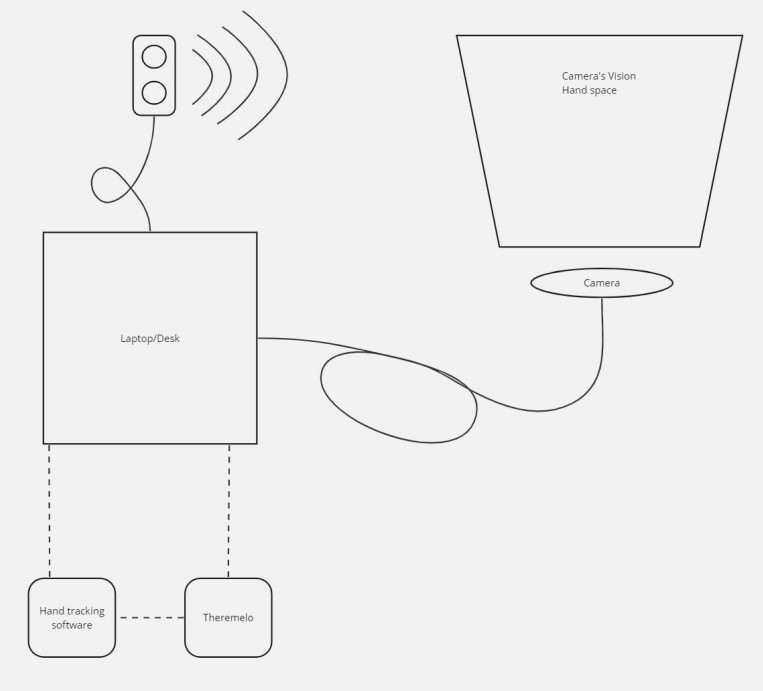
\includegraphics[width=0.8\textwidth]{images/systemOverview.jpg}
    \caption{System Overview}
\end{figure}
